%%%%%%%%%%%%%%%%%%%% author.tex %%%%%%%%%%%%%%%%%%%%%%%%%%%%%%%%%%%
%
% sample root file for your "contribution" to a contributed volume
%
% Use this file as a template for your own input.
%
%%%%%%%%%%%%%%%% Springer %%%%%%%%%%%%%%%%%%%%%%%%%%%%%%%%%%%%%%%%%


%% RECOMMENDED %%%%%%%%%%%%%%%%%%%%%%%%%%%%%%%%%%%%%%%%%%%%%%%%%%%
%\documentclass[graybox]{svmult}
%
%% choose options for [] as required from the list
%% in the Reference Guide
%
%\usepackage{mathptmx}       % selects Times Roman as basic font
%\usepackage{helvet}         % selects Helvetica as sans-serif font
%\usepackage{courier}        % selects Courier as typewriter font
%\usepackage{type1cm}        % activate if the above 3 fonts are
%                           % not available on your system
%
%\usepackage{makeidx}         % allows index generation
%\usepackage{graphicx}        % standard LaTeX graphics tool
%                             % when including figure files
%\usepackage{multicol}        % used for the two-column index
%\usepackage[bottom]{footmisc}% places footnotes at page bottom
%\usepackage{mathtools}
%\mathtoolsset{showonlyrefs}
%
%% see the list of further useful packages
%% in the Reference Guide
%
%\makeindex             % used for the subject index
%                       % please use the style svind.ist with
%                       % your makeindex program
%
%%%%%%%%%%%%%%%%%%%%%%%%%%%%%%%%%%%%%%%%%%%%%%%%%%%%%%%%%%%%%%%%%%%%%%%%%%%%%%%%%%%%%%%%%%
%
%\begin{document}

\title{Global search algorithms for one-dimensional multiextremal optimization problems with nonlinear constraints}
% Use \titlerunning{Short Title} for an abbreviated version of
% your contribution title if the original one is too long
\author{Name of First Author and Name of Second Author}
% Use \authorrunning{Short Title} for an abbreviated version of
% your contribution title if the original one is too long
\institute{Name of First Author \at Name, Address of Institute, \email{name@email.address}
\and Name of Second Author \at Name, Address of Institute \email{name@email.address}}
%
% Use the package "url.sty" to avoid
% problems with special characters
% used in your e-mail or web address
%
\maketitle

\abstract{The chapter considers a method for reduction of a constrained problem to an
unconstrained one, so called \emph{index method}. This method, unlike the classical penalty function
one, allows avoiding the problem of the parameter selection (like the penalty coefficients for the
constraints) and also allows solving the problems with so called partially defined constraints,
which could not be solved by any other method. The serial and parallel algorithms for solving
univariate problems are considered.}

\keywords{multiextremal optimization, nonconvex constraints, index method, parallel
algorithms}

\section{Problem statement}
In the present chapter, the one-dimensional problems of the constrained optimization will
be considered. Let $\varphi(x)$ and $g_j(x)\le 0,1\le j\le m$ be the real functions defined in a closed interval $[a,b]$ of the real axis. It is requires to find the values $x^*$ satisfying the condition
\begin{equation}
  \label{eq4:problem}
  \varphi(x^*)=\min\{\varphi(x):x\in [a,b], g_j(x)\le 0,1\le j\le m\}
\end{equation}

As before, the objective function $\varphi$ (hereinafter denoted also as $g_{m+1}$) and the left parts of the constraints $g_j(x)\le 0,1\le j\le m$ re assumed to satisfy \emph{Lipschitz condition} with the corresponding constants $L_j,1\le j\le m+1$, namely:
\begin{equation}
  |g_j(x_1)-g_j(x_2)|\le L_j|x_1-x_2|,1\le j\le m+1,x_1,x_2
\end{equation}

\example{
\label{ex4:problem}
Let us consider a problem of type \eqref{eq4:problem} where $x\in [0.6;2.2],m=2$,
\begin{gather}
  \varphi(x)=\cos(18x-3)\sin(10x-7)+1.5, \\
  g_1(x)=\exp(-x/2)\sin(6x-1.5), \\
  g_2(x)=|x|\sin(2\pi x-0.5).
\end{gather}
he exact solution of the problem is $x^*=2.0795,\varphi(x^*)=0.565$. The graphs of the functions $g_1(x),g_2(x)$,and $\varphi(x)$ are presented in Fig. \ref{fig:4_1}.
\begin{figure}[h]
  \label{fig:4_1}
  \centering
  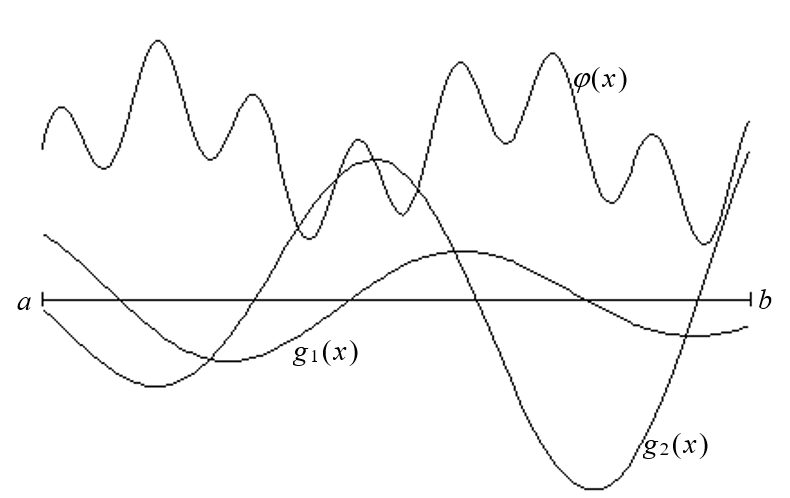
\includegraphics[width=0.8\textwidth]{figures/4_1.png}
  \caption{One-dimensional global optimization problem}
\end{figure}
}

\section{Partial computability and index scheme of the account of constraints}
Problem \eqref{eq4:problem} can be considered in the statement when each function $g_j,1\le j\le m+1$ is defined and computable only in the corresponding subdomains $Q_j\subset [a,b]$ where
\begin{equation}
  \label{eq4:q}
  Q_1=[a,b],Q_(j+1)=\{x\in Q_j:g_j(x)\le 0\},1\le j\le m.
\end{equation}

For example, in the optimal design problems some characteristics of the technical systems may appear to be undefined if the conditions of the system functioning represented by a part of the constraints of problem \eqref{eq4:problem} are not fulfilled.

Taking into account conditions \eqref{eq4:q}, initial problem \eqref{eq4:problem} can be represented in the form
\begin{equation}
  \varphi(x^*)=\min\{g_{m+1}(x):x\in Q_{m+1}\}.
\end{equation}

For the purposes of further treatment, let us introduce a classification of the points $x$ in the search domain $[a,b]$ using an index $\nu=\nu(x)$ where $\nu-1$ is the number of constraints, which are fulfilled in this point. Formally, the index $\nu$ is defined by the conditions
\begin{equation}
  g_j(x)\le 0,1\le j \le \nu-1,g_\nu(x)>0,
\end{equation}
(the last inequality is inessential  if $\nu=m+1$) and it satisfies the inequalities
\begin{displaymath}
  1\le\nu=\nu(x)\le m+1.
\end{displaymath}
The problem of example \ref{ex4:problem} assuming a partial computability of the functions is presented in Fig. \ref{fig:4_2}. The arcs of the restrictions $g_1(x),\:g_2(x)$, and of the objective function $\varphi(x)$ defined in the corresponding subdomains $Q_j$ from \eqref{eq4:q} are shown. The point $x^1$ with the index $\nu(x^1)=1$, the point $x^2$ with the index $\nu(x^2)=2$, and the point $x^3$ with the index $\nu(x^3)=3$ are shown also.

\begin{figure}[h]
  \label{fig:4_2}
  \centering
  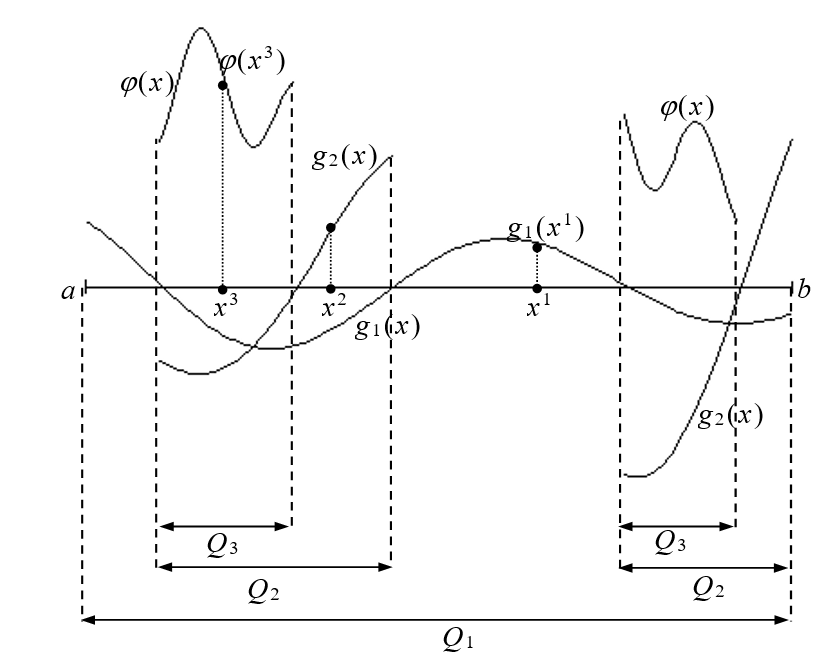
\includegraphics[width=0.8\textwidth]{figures/4_2.png}
  \caption{A problem with partially computable functions}
\end{figure}

This classification generates the function
\begin{equation}
  \label{eq4:fx}
  f(x)=g_\nu(x),\nu=\nu(x),
\end{equation}
defined and computable everywhere in $[a,b]$. Its value at a point $x$ is either the value of the left part of the constraint violated at this point (the case $\nu\le m$)  or the value of the objective function (the case $\nu=m+1$). Therefore, the determination of the value of $f(x),\:x\in[a,b]$  is reduced to a successive computations of the values of $g_j(x), 1\le j\le \nu=\nu(x)$, i.e., the next value $g_{j+1}(x)$ is calculated in the case when $g_j(x)\le 0$ only. The computational process finishes either as a result of the fulfillment of the inequality $g_j(x)>0$ or as a result of achievement of the value $\nu(x)=m+1$.

The described procedure called a \emph{trial} at the point $x$ forms the index $\nu$ of this point automatically. The pair of values
\begin{equation}
  z=f(x)=g_\nu(x),\nu=\nu(x)
\end{equation}
generated by the trial at the point $x\in[a,b]$ is called the \emph{trial result}.

The graph of the function $f(x)$ from \eqref{eq4:fx}, which consists of the arcs of the constraints $g_1(x),\:g_2(x)$, and of the objective function $\varphi(x)$ taken from Example \ref{ex4:problem} is shown in Fig. \ref{fig:4_3}.

\begin{figure}[h]
  \label{fig:4_3}
  \centering
  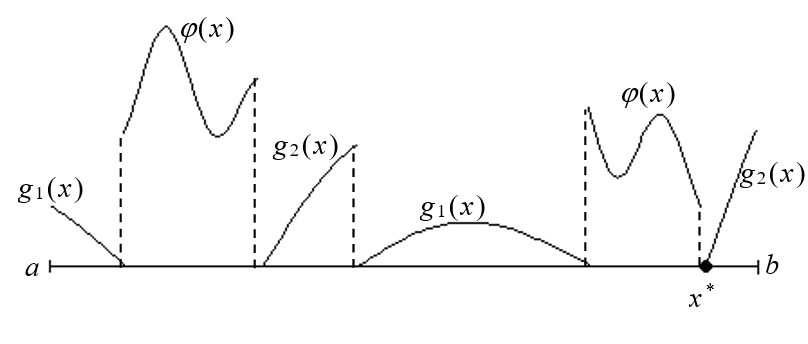
\includegraphics[width=0.8\textwidth]{figures/4_3.png}
  \caption{An «index» function}
\end{figure}

%\end{document}
